
\section{Multi-Phase Generation Techniques at mm-Wave Frequencies}
At frequencies above 10\,GHz, eight evenly-spaced phases are typically realised with either delay-locked loops (\glspl{dll}), ring oscillators or phase-interpolation \gls{pi} networks, each option presenting a distinct set of trade-offs in jitter, resolution and power.

\subsection{DLL-based generation}
A conventional \gls{dll} cascades $N$ voltage- or digitally-controlled delay cells whose total delay is phase-locked to one input period, thereby providing $N$ equi-spaced taps \cite{Wang2021JSSC}.

In advanced nodes, achieving high timing resolution is critical; for instance, the need for sub-picosecond step sizes is paramount in high-speed timing circuits, especially for elements like \gls{pi} which require very fine resolution \cite{Mishra2022ISSCC}.
Jitter accumulates along the chain, thus recent \gls{dll} embed mixed-signal calibration or injection-locked buffers to suppress noise.

\subsection{Ring oscillators and injection locking}
An $N$-stage ring oscillator inherently delivers $N$ phase outputs but suffers from inferior phase noise compared with LC tanks. Injecting a clean multi-phase reference periodically forces the ring to lock, yielding jitter suppression while preserving compact CMOS realisation \cite{Wang2021JSSC}.

Hybrid quadrature-DLL plus injection-locked ring topologies achieve $<\!1^{\circ}$ phase error and sub-60\,fs rms jitter at 7–8\,GHz \cite{Wang2021JSSC}, establishing a blueprint for mm-wave multi-phase clocks.

While highly effective, the performance of an injection-locked oscillator is sensitive to the properties of the injection signal itself. The final phase accuracy can be degraded by mismatches in the amplitude and phase of the multi-phase injection inputs, a critical consideration for achieving low phase error in practical implementations \cite{Wang2025ArXiv}.

\subsection{Phase interpolation}
Where only a subset of base phases is available, additional phases can be synthesised by weighted mixing of two inputs.
For instance, a modern 9-bit integrating-mode \gls{pi} in 5\,nm FinFET operates with a frequency range of 9-14\,GHz, achieving \SI{295}{\femto\second} \gls{dnl}$_{pp}$ (Differential Non-Linearity) and consuming approximately 0.43\,mW/GHz \cite{Mishra2022ISSCC}. In another example, an 8-bit ramp-based \gls{pi} in 65\,nm CMOS provides 0.8\,least-significant bit(\gls{lsb}) differential non-linearity(\gls{dnl})$_{p-p}$ over a 6-12\,GHz range with a power efficiency of 0.18\,mW/GHz \cite{Mohapatra2024ISSCC}.

Scaling to advanced nodes like 3\,nm continues, with reported \gls{pll} operating in the 12.6-14.5\,GHz range \cite{Lu2022JSSC}; however, specific performance expectations for multi-phase generators at such nodes, such as extending operating ranges to 22.5\,GHz, would depend on dedicated designs and characterizations. General challenges in such scaled nodes include managing increased device variability and routing parasitics.
Symmetric layout, common-centroid strategies and on-chip calibration remain mandatory to combat phase skew and duty-cycle distortion.


\section{Programmable Delay Elements}
Programmable delay elements (\glspl{pde}) are crucial for adjusting signal paths to correct skew introduced by systematic jitter, temperature variations, or process variations, which become increasingly critical as process nodes shrink~\cite{horowitz2005scaling, caignet2001challenge, lee2011self, Park2021, abdulrazzaq2016review}. The most common implementations of \gls{pde} are based on current-starving, parallel NMOS capacitors, tapped delay lines, and inverter matrices.

\subsection{Current-starved delay elements}
The propagation delay of a CMOS gate is inversely proportional to the charging/discharging current available for the load capacitance.  A current‑starved inverter (\gls{csi}) exploits this fact by inserting one or more limiter transistors in series with the pull‑up and/or pull‑down devices of a minimum‑size inverter; the limiter(s) throttle the current, thereby stretching or shrinking the delay~\cite{maymandi2003digitally}.  Because the underlying inverter is compact and its delay model is well understood, \glspl{csi} are widely used in delay‑locked loops, VCOs and digitally‑controlled delay lines.

There are two common ways to program the delay:
\begin{enumerate}[label=\alph*]
  \item \textbf{Analog (voltage‑controlled) \gls{csi}.}\\
        A single NMOS (and/or PMOS) limiter is added in series, and an analog control voltage~$V_{\mathrm{ctrl}}$ applied to its gate sets the channel current continuously.  In practice $V_{\mathrm{ctrl}}$ is often produced off‑chip or by an on‑chip DAC; once delivered to the \gls{csi} it is a true analog bias.  This offers sub‑20\,fs resolution in advanced nodes, limited mainly by the $V_{\mathrm{ctrl}}$ step size and noise~\cite{Batur2015high}.  The drawback is strong non‑linearity of the transistor transfer characteristics (\(ID-V_{GS}\)) (that follow square‑law in saturation and exponential in sub‑threshold) and process/temperature sensitivity, which complicate open‑loop calibration~\cite{Seraj2015new}.
  \item \textbf{Digitally‑switched \gls{csi}.}\\
        Instead of a single limiter, $N$ limiter transistors of equal or binary‑weighted width are placed in parallel.  Each gate is hard‑wired to either~$V_{\mathrm{DD}}$ or~0 by a digital control bit, effectively switching that current path fully on or completely off~\cite{maymandi2005monotonic,yao2011}.  This realises a unary or binary‑weighted current digital to analog converter (\gls{dac}) in the current domain and yields a step‑wise (but monotonic) delay curve.  The resolution is set by the minimum device width; the \gls{lsb} delay step is typically tens of femtoseconds in modern CMOS~\cite{Heck2015optimization}.  Monotonicity is easier to guarantee than in analog \gls{csi}, but the total device area and parasitic capacitance rise with the number of bits.
\end{enumerate}

Figure~\ref{fig:csi_delay_eg} shows a representative \gls{csi} using four parallel PMOS transistors~(M1--M4) and a subsequent current mirror as a simple \gls{dac}, generating the control voltage at the pull-down NMOS gate. When more control bits are asserted, the voltage at the pull-down transistor's gate increases, increasing the pull‑down current and shortening the falling‑edge delay. De‑asserting bits has the opposite effect. An analogous network may be placed in the pull‑up path for symmetric control of the rising edge.

Current-starved delay elements have some limitations, including non-linearity and asymmetry, resolution limits, and speed penalties.

Because NMOS and PMOS devices have different mobility and threshold voltages, their I--V characteristics, and hence the incremental delay change, are unequal.  Without compensation, the rising/falling delays may diverge, degrading duty‑cycle and phase‑noise performance~\cite{Heck2015optimization}.  Tightening the $V_{\mathrm{ctrl}}$ range (analog \gls{csi}) or adding extra tuning bits only for the slower edge (digital \gls{csi}) partially mitigates this at the cost of tuning range and complexity.

In analog CSIs, resolution is bounded by the smallest reproducible $V_{\mathrm{ctrl}}$ step, DAC INL/DNL and on‑chip noise.  In digitally‑switched CSIs it is bounded by the minimum transistor width and the parasitic capacitance added by each extra limiter device.


\begin{figure}[hb]
    \centering
    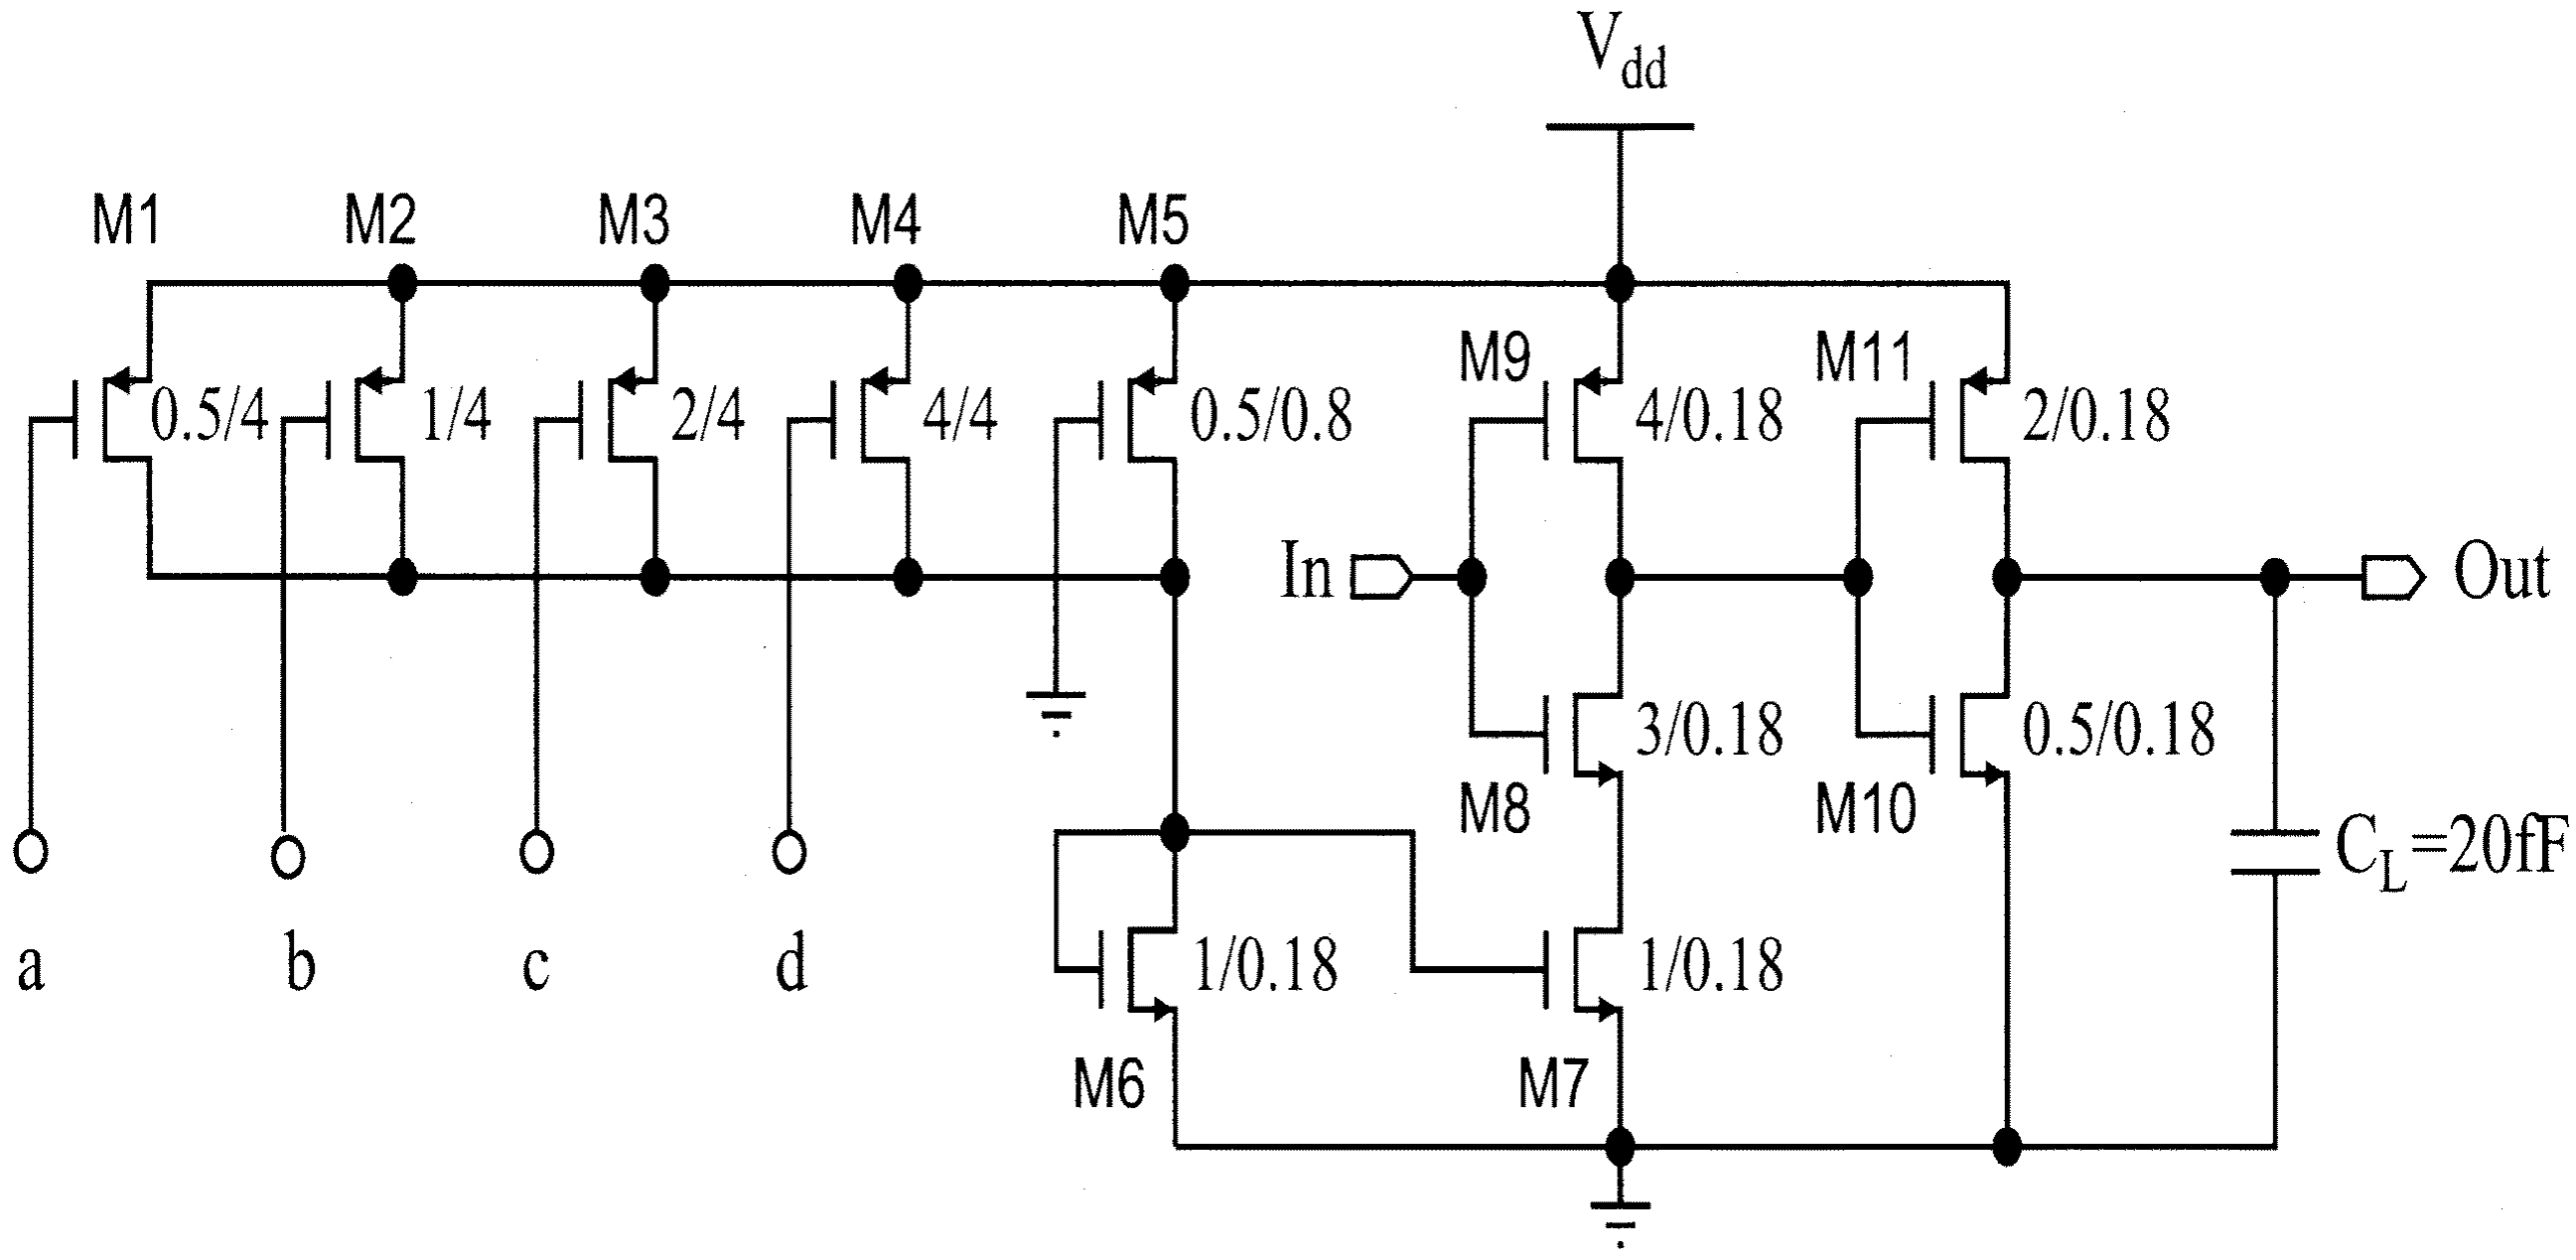
\includegraphics[width=0.7\textwidth]{figures/Schematics/CSI_delay_example.png}
    \caption{Example of a \gls{csi} delay element in 180\,nm CMOS. Replicated from~\protect\cite{maymandi2003digitally}}\label{fig:csi_delay_eg}
\end{figure}

\subsection{Shunt Capacitor}
This technique is based on the fact that the delay of a digital cell is proportional to the capacitance at its output, as described by the time constant $ \tau = R \cdot C $. By increasing the capacitance, the delay can be increased, and vice versa.
MOS capacitors operating in accumulation mode can provide a linear capacitance $C_{ox}\approx C_{vgs}$. Capacitance is adjusted either by controlling the gate voltage or by switching binary-weighted arrays in and out of the signal path~\cite{andreani1998shunt}.
This technique is highly linear and has the possibility of introducing very low jitter if passive components are used, though it suffers from large area overhead owing to the large size of MOS capacitors~\cite{pao2005portable}.

Figure~\ref{fig:sci_delay_eg} shows an example of a shunt capacitor delay element, where the capacitance is adjusted by switching in and out binary-weighted capacitors. The output voltage will, ideally, behave as a regular capacitor charge ramp, given by the equation $ V_{out} = V_{in} \cdot (1 - e^{-t/RC}) $, where $ R $ is the resistance and $ C $ is the capacitance. Here, the capacitance is digitally programmable as \(C = \sum_{i=1}^{N} C_i \cdot S_i\), meaning the output voltage (dis)charge is controlled by the digital input.

\begin{figure}[htbp]
    \centering
    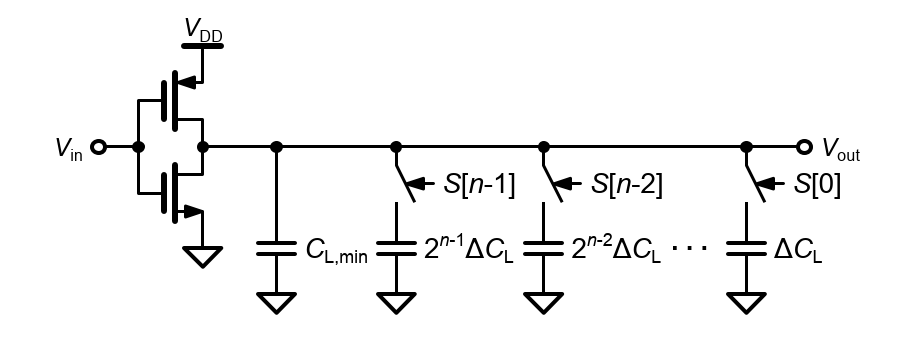
\includegraphics[width=0.7\textwidth]{figures/Schematics/SCI_delay_example.png}
    \caption{Example of a SCI delay element. Replicated from~\protect\cite{Angeli_2018}}\label{fig:sci_delay_eg}
\end{figure}

Some novel circuits have been proposed to address the area overhead of shunt capacitor delay elements, such as the use of switched capacitor arrays~\cite{Ramazanoglu2018switched}. These designs are more complex and require careful design to ensure proper operation.

\section{State-of-the-Art overview}
Table~\ref{tab:sota_summary_enhanced} compares eight representative multi-phase clock–generation and digitally–programmable delay solutions published between 2018 and 2025. The designs span $3,$nm–$65,$nm CMOS/FinFET processes and cover a fundamental frequency range from $2,$GHz to $28,$GHz, thereby embracing the entire spectrum required for quarter-, half- and full-rate wire-line \gls{serdes} links up to (and beyond) $112,$Gb/s.

Many recent prototypes adopt injection-locked or multi-phase ring-oscillator cores to naturally deliver eight evenly spaced phases. \gls{pi}-assisted variants further trim the timing step, achieving sub-picosecond resolution as seen in \cite{Mishra2022ISSCC}. \gls{rms} jitter has shown marked improvement, falling from $148,$fs in 2020 \cite{Chen2020VLSIC} to just 38~fs in 2025 \cite{Tian2025ISSCC} over comparable integration bandwidths. Meanwhile, the active area has been pushed below 0.01\(mm^2\) through aggressive technology scaling, reaching a minimum of 0.0017\(mm^2\) \cite{Chen2020VLSIC}.

Power dissipation still varies widely, from a low of $2.2,$mW in a ramp-based \gls{pi} \cite{Mohapatra2024ISSCC} to $90,$mW in a wide-tuning ring oscillator \cite{Tian2025ISSCC}, reflecting different target jitter specifications and on-chip power constraints.

A widely adopted Figure of Merit that normalizes performance based on RMS jitter ($\sigma_j$) and DC power consumption ($P_{DC}$) was also determined for all references presented in the table, calculated as $10 \log_{10} ((\sigma_j / 1s)^2 \cdot (P_{DC} / 1mW))$. A lower (i.e., more negative) value indicates better performance. Adapted from \cite{Lu2022JSSC}.

\begin{table*}[h]
 \caption{Comparison of Multi-Phase Clock Generators and Delay Elements.}
 \label{tab:sota_summary_enhanced}
 \centering
 \resizebox{\textwidth}{!}{%
 \begin{tabular}{@{}l l c S[table-format=1.2] c c c S[table-format=2.1] S[table-format=1.3] S[table-format=1.2] c S[table-format=-3.1] S[table-format=-3.1] @{}}
  \toprule
  \textbf{Reference} & \textbf{Tech.} & \textbf{Freq.} & {\textbf{Supply}} & \textbf{Phases} & \textbf{Resolution} & \textbf{Jitter} & {\textbf{Jitter BW}} & {\textbf{DNL/INL}} & {\textbf{Power}} & \textbf{Area} & {\textbf{Power Eff.}} & {\textbf{FoM\textsubscript{J}}} \\
   & & \textbf{(GHz)} & {\textbf{(V)}} & & & \textbf{(fs\textsubscript{rms})} & {\textbf{(MHz)}} & {\textbf{(fs or LSB)}} & \textbf{(mW)} & \textbf{(mm\textsuperscript{2})} & {\textbf{(mW/GHz)}} & {\textbf{(dB)}} \\
  \midrule

  Chen '18 \cite{Chen2018ISSCC} & 7nm FinFET & 4--16 & 1.2/0.88 & 8 (+PI) & 7-bit PI & 80\textsuperscript{a} & {0.1--1k} & {0.87/1.44LSB} & 22.4 & 0.105 & 1.40 & -248.4 \\

  Song '19 \cite{Song2019CICC} & 16nm FinFET & 2--20 & 1/0.863 & 8 & 6-bit PI & {---}\textsuperscript{b} & {---} & {0.7/1.6LSB} & 43 & 0.0036 & 2.15 & {---} \\

  Chen '20 \cite{Chen2020VLSIC} & 5nm FinFET & 4--18 & 1 & 4 & 6-bit QEC & 148\textsuperscript{c} & {0.1--1k} & {---} & 21\textsuperscript{d} & 0.0017 & 1.17 & -243.4 \\

  Wang '21 \cite{Wang2021JSSC} & 65nm CMOS & 5--8 & 1.2 & 8 & 7-bit PI & 58.8 & {0.1--1k} & {1.2/1.9} & 15.6\textsuperscript{e} & 0.021 & 1.95 & -252.7 \\

  Lu '22 \cite{Lu2022JSSC} & 3nm FinFET & 12.6--14.5 & 0.875 & PLL & PLL & 56\textsuperscript{f} & {0.001--100} & {---} & 18.6 & 0.045 & 1.28 & -252.3 \\

  Mishra '22 \cite{Mishra2022ISSCC} & 5nm FinFET & 9--14 & 0.75 & PI & 9-bit & 71 & {3--3k} & {295fs/510fs} & 6 & 0.006 & 0.43 & -255.2 \\

  Mohapatra '24 \cite{Mohapatra2024ISSCC} & 65nm CMOS & 6--12 & 1.2 & 4/2 (PI) & 8-bit & 68 & {0.1--1k} & {0.8/1.7LSB} & 2.2 & 0.025 & 0.18 & -258.8 \\

  Tian '25 \cite{Tian2025ISSCC} & 28nm CMOS & 8--28 & 1.1 & 8 & $3^{\circ}$ error & 38\textsuperscript{g} & {0.001--1k} & {---} & {26--90} & 0.02 & 3.21 & -254.4\textsuperscript{h} \\

  \bottomrule
 \end{tabular}
}
\vspace{0.5em}
\begin{minipage}{\textwidth}
\footnotesize
 \textsuperscript{a}Full clock chain jitter @16GHz.
 \textsuperscript{b}RMS jitter for generator not reported.
 \textsuperscript{c}Integrated @18GHz.
 \textsuperscript{d}QCG only. Full path consumes 37mW.
 \textsuperscript{e}For QDLL+MPILOSC core.
 \textsuperscript{f}Integrated @13.28GHz.
 \textsuperscript{g}Includes signal source noise.
 \textsuperscript{h}Calculated at maximum power (90mW).
\end{minipage}
\end{table*}
